%%---------------------------------------------------------------------
%	Preamble
%	AMS gruppe 12
%	AMS F18
%---------------------------------------------------------------------
\documentclass[12pt,fleqn,a4paper]{article}
\usepackage[utf8]{inputenc}
\usepackage[danish]{babel}
\usepackage[top=2.5cm, left=2cm, right=2cm, bottom=2.5cm]{geometry}
\usepackage{graphicx}
\usepackage[bottom]{footmisc}
\usepackage{framed}
\usepackage{caption}
\usepackage{float}
\usepackage{mdframed}
\usepackage{listings}
\usepackage{color}
\usepackage[T1]{fontenc}
\usepackage{amsmath,amsfonts,amsthm} % Math packages
\usepackage{array}
\usepackage{wrapfig}
\usepackage{multirow}
\usepackage{tabu}
\usepackage{longtable}
\usepackage{lastpage}
\usepackage{fancyhdr}
\usepackage[compact]{titlesec}
\usepackage[table,xcdraw]{xcolor}
\usepackage{arydshln}
\usepackage[isbn,issn,url]{dk-bib}
\usepackage[toc,page]{appendix}
\usepackage{url}
\def\UrlBreaks{\do\/\do-}

\definecolor{mygreen}{RGB}{28,172,0} % color values Red, Green, Blue
\definecolor{mylilas}{RGB}{170,55,241}
\renewcommand{\lstlistingname}{Kodeudsnit}
\tabulinesep=3mm

\setcounter{secnumdepth}{2}
\setcounter{tocdepth}{2}

\setlength{\parindent}{0mm} %intet indryk
\setlength{\parskip}{3mm} 	%linjeskift v. afsnit

% Ændring af enumerize og itemize 
\usepackage{enumitem} % @http://ctan.org/pkg/enumitem
\setlist[itemize]{topsep=0pt, itemsep=0.5pt}
\setlist[enumerate]{topsep=0pt, itemsep=0.5pt}

%afstand omkring sections
\titlespacing{\section}{0pt}{5mm}{0pt}
\titlespacing{\subsection}{0pt}{2mm}{0pt}
\titlespacing{\subsubsection}{0pt}{2mm}{0pt}

\usepackage{arydshln}
%aryd
\setlength\dashlinedash{3pt}
\setlength\dashlinegap{4pt}

\lstset{language=C++,
	breaklines=true,
	keywordstyle=\color{blue},
	stringstyle=\color{red},
	commentstyle=\color{mygreen},
	morecomment=[l][\color{magenta}]{\#}
}

%header & footer
\makeatletter
\pagestyle{fancy}
\fancypagestyle{plain}{}
\renewcommand{\chaptermark}[1]{\markboth{#1}{}}
\setlength{\headheight}{35pt}
\fancyfoot{} % clear all fields
\fancyfoot[R]{Side \thepage\ af \pageref{LastPage}}
\fancyhead{} % clear all fields
\fancyhead[L]{
\includegraphics[clip, trim = 0 0 240pt 0, height=30pt]{Figur/IHA_AU_logo.png}}
\fancyhead[R]{Forår 2018}
\fancyhead[C]{Anvendte Microcontroller Systemer}
\renewcommand{\headrulewidth}{0pt}

\def\thickhrulefill{\leavevmode \leaders \hrule height 1.2ex \hfill \kern \z@}
\def\@makechapterhead#1{
  \vspace*{10\p@}%
  {\parindent \z@ \centering \reset@font
        \thickhrulefill\quad 
        \scshape\bfseries\textit{\@chapapp{}  \thechapter}  
        \quad \thickhrulefill
        \par\nobreak
        \vspace*{10\p@}%
        \interlinepenalty\@M
        \hrule
        \vspace*{10\p@}%
        \Huge \bfseries #1 \par\nobreak
        \par
        \vspace*{10\p@}%
        \hrule
        \vskip 40\p@
  }}

\usepackage{tcolorbox}
\definecolor{mycolor}{rgb}{0.122, 0.435, 0.698}% Rule colour
\makeatletter
\newcommand{\mybox}[1]{%
	\setbox0=\hbox{#1}%
	\setlength{\@tempdima}{\dimexpr\wd0+13pt}%
	\begin{tcolorbox}[colframe=mycolor,boxrule=0.5pt,arc=4pt,
		left=6pt,right=6pt,top=6pt,bottom=6pt,boxsep=0pt]
		#1
	\end{tcolorbox}
}
\makeatother

\graphicspath{ {Figur/} }


%Se Kodeudsnit \ref{lstlisting:generel_kode}

%\captionof{lstlisting}{Generelle egenskaber for koden til fremstilling af diverse figure i matlab} 
%\label{lstlisting:generel_kode}
%\vspace{5mm} %5mm vertical space
%
%\subsection{Kode til lyd i forhold til tiden}
%\begin{framed}
%\begin{center}
%\begin{lstlisting}
%figure('name','trafikstoejen i fuld laengde'); clf
%subplot(211);
%plot(t,s_sound_left)
%xlabel('Tid (sek)')
%ylabel('Signalstyrke')
%title('Trafikstoej set i forhold til tiden')
%grid on
%hold on
%\end{lstlisting}
%\end{center}
%\end{framed}




%\begin{document}

\section{Øjendetekteringsmodul}

I det følgende afsnit vil øjendetektionensmodulets design og implementering, samt test heraf blive beskrevet. 

Øjendetekteringsmodulet er en del af den PC-software som EyeRobot indeholder. Modulets ansvar er at omsætte et videofeed til styringskommandoer, som bruges til at navigere GUI'et.
Set fra et ”black box view” skal modulet forstås med in- og output som vist på figur \ref{fig:eyetrack_modulbeskrivelse}.

\begin{figure}[H] 
\centering
	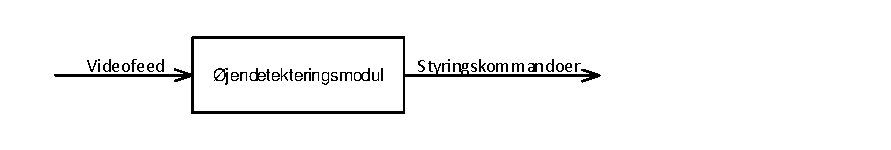
\includegraphics[width =0.8 \textwidth]{Figur/eyetrack_modulbeskrivelse.pdf}
	\captionof{figure}{modul view af øjendetekteringssektionen}
	\label{fig:eyetrack_modulbeskrivelse}
\end{figure}

Videofeedet hentes fra et kamera rettet mod brugerens ansigt, men det er også muligt at sende en videofil gennem modulet til testformål.
Øjendetekteringsmodulet står for detektering, samt kalkulering af brugerens synsretning. 
Øjendetekteringsmodulet er udviklet som en lukket boks med grænseflader til resten af systemet. \\
Modulet er designet til at køre med sit eget hovedforløb, hvorfra der kan hentes den detekterede øjeretning, når modulet tillader det. 
Dette er implementeret ved at lade modulet køre i sin egen tråd og kommunikere med udefrakommende software via en blokerende get-metode. 

\subsection{Foranalyse}
\subsubsection{Software analyse}
Til øjendetekteringsmodulet skal der bruges et bibliotek som indeholder implementeringer af de metoder, som skal bruges til detektering og behandling af videoframes. 
Af krav til biblioteket er: God dokumentation, nem integration med anden software og realtidsegenskaber. 
Der er fundet to mulige kandidater, OpenCV og Matlab, som kan løfte opgaven. 
Der er god dokumentation for begge dele, samt mulighed for realtidshåndtering. 
OpenCV er skrevet i C++ og er optimeret til realtid, dette gør OpenCV til det oplagte valg, da resten af applikationen også er skrevet i C++. 
Af disse grunde er OpenCV version 2.4.9 valgt.  

\subsubsection{Hardware analyse}
I forbindelse med øjendetekteringsmodulet er der overvejet tre mulige detekteringsmetoder, hver metode stiller hver sit krav til hardware:

\begin{enumerate}
	\item Ansigts- og øjendetektering som reference til pupil koordinater 
	\item Pupil center corneal reflection tracking 
	\item Hovedmonteret kamera
\end{enumerate}

I den første løsning består hardwaren af et simpelt kamera, der kan levere et videofeed som input til øjendetekteringsmodulet. 
Dette input bruges til billedbehandling, hvor der køres detekteringsalgoritmer til at finde ansigtet og øjnene på brugeren. 
Øjnene bruges som reference til at finde pupilkoordinater.
Kameraet hertil behøver kun at være et standard webcam.

Den anden løsning, pupil center corneal reflection tracking, som er en udvidelse af den første løsning, og kræver hardware i form af et infrarødt kamera og en infrarød lyskilde. 
Ved brug af infrarødt lys, dannes en refleksion i pupillen, som kameraet kan opfange. 
Med refleksionen som reference gives mulighed for en mere præcis aflæsning af pupillens koordinater, hvilket nedsætter signalbehandlingen. 
Denne løsning er også en standard indenfor øjendetekteringsprodukter, men ulempen er de ekstra hardware komponenter der kræves.

Den tredje løsning er at bruge et hovedmonteret kamera, hvilket kræver, at der udvikles en monteringsløsning i form af et headset eller en hjelm. 
Fordelen ved dette er, at referencen i forhold til pupillen er konstant, men ulempen er at udforme en designløsning, der ikke begrænser brugerens synsfelt og mulighed for at se GUI'et.

For at mindske ekstraudgifter, og derved gøre produktet lettere tilgængeligt, er den første løsning valgt. 
Vurderingen er også taget ud fra, hvilket krav systemet har til præcisionen af detekteringen.
Hvor standardøjendetekteringsprodukter har til formål, at erstatte en mus, har Eyerobot sin egen grafiske brugerflade, hvor de valgfelter brugeren anvender til at navigere rundt i systemet er gjort så store, at en mindre præcision kan accepteres.


\subsection{Antagelser i implementeringen} 
Der er mange metoder, hvorved information om en brugers synsretning kan udregnes.
I dette afsnit forklares, hvilke antagelser, som er gjort i EyeRobots tilgang til implementeringen af funktionaliteten. 
De grundlæggelse antagelser er listet herunder:   
 
	\begin{enumerate}
  	\item Det detekterede øjecentrum afhænger ikke af synsretningen.
  	\item Øjet er repræsenteret med nok pixels således, at referencer kan beregnes.
  	\item Iris er det mørkeste objekt i billedet.
 	\item Det største ansigt i et frame er det styrende ansigt. 
	\end{enumerate}

Med første punkt menes, at den anvendte metode til at lokalisere øjet ikke forskyder øjets centrum i forhold til pupillens position. 

Dernæst er det vigtigt, at opløsningen er fin nok til, at iris' position kan skelnes fra øjets centrum, som det ses på figur \ref{fig:irisdetectbeskrivelse}. 

\begin{figure}[H]
	\centering
	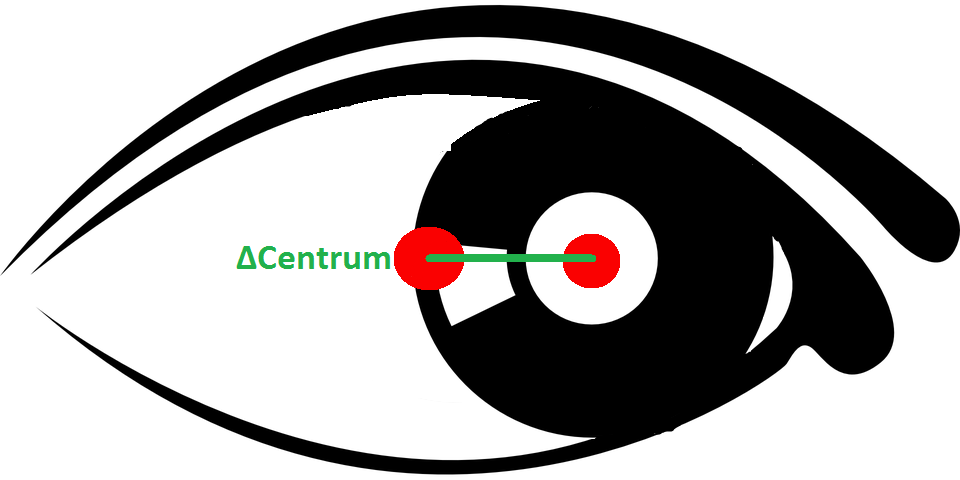
\includegraphics[width=0.45 \textwidth]	 {irisdetectbeskrivelse2.png}
	\captionof{figure}{Konceptbillede af irisdetekt}
	\label{fig:irisdetectbeskrivelse}
\end{figure}

Iris' position bliver fortolket i de fem forskellige områder som vist på figur \ref{fig:irisdetectbeskrivelsefelter}.                          

\begin{figure}[H]
	\centering
	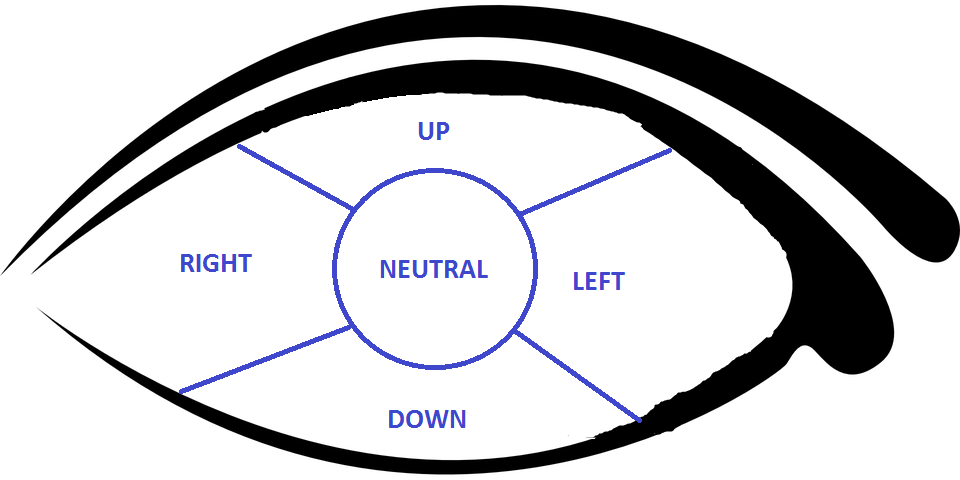
\includegraphics[width=0.45 \textwidth]	 {eyeregiondescription.png}
	\captionof{figure}{Konceptbillede af inddeling af felter i øjet}
	\label{fig:irisdetectbeskrivelsefelter}
\end{figure}


\subsection{Flowbeskrivelse for Øjendetekteringsmodul}
Figur \ref{fig:mainflowdiagram} viser et flowdiagram, for modulets overordnede funktionalitet. \\
I kalibreringen bestemmes det om der er en bruger (et ansigt), samt om øjnene kan detekteres. 
Her vælges også et af brugerens øjne, som vil blive brugt til at finde synsretningen ud fra. 
Der kalibreres også for lysintensitet. \\

\begin{figure}[H]
	\centering
	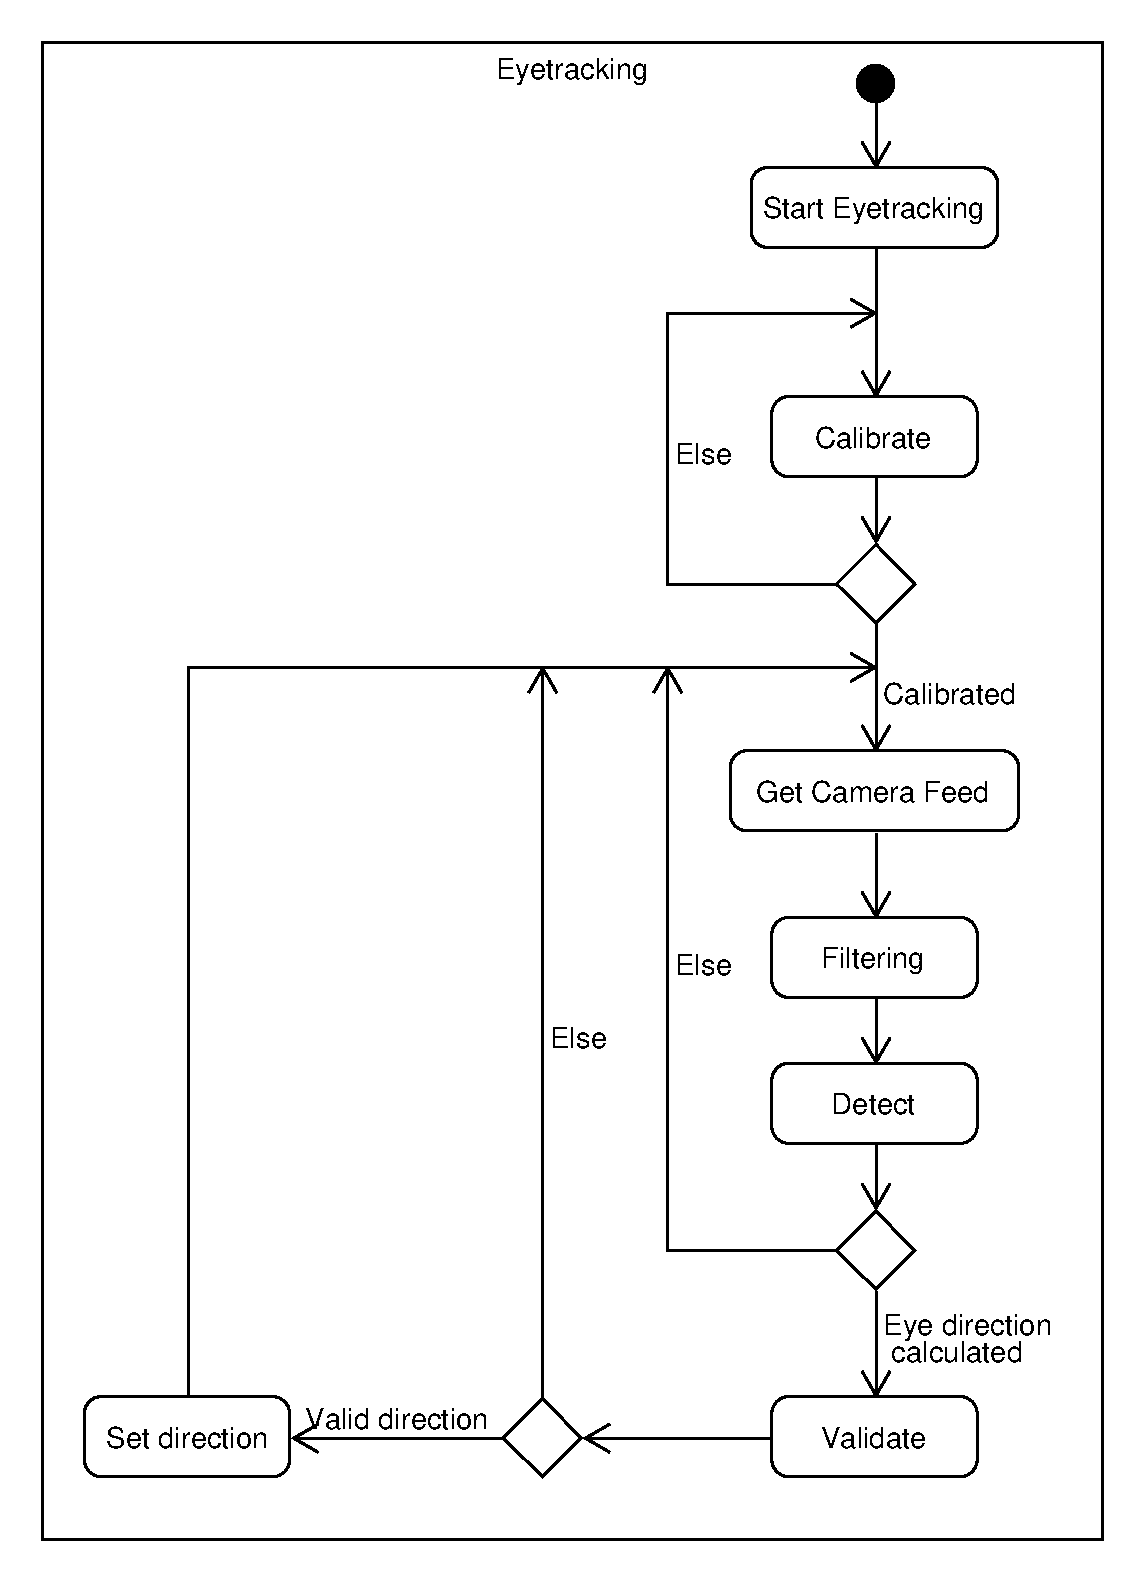
\includegraphics[clip, trim = 0cm 0cm 0cm 0cm ,width =0.6 \textwidth] {EyeTrackMainFlow.pdf}
	\captionof{figure}{Flowdiagram over eyetracking mainflow}
	\label{fig:mainflowdiagram}
\end{figure}

Efter kalibrering begynder hovedloopet, som består af tre blokke. 
Mellem hver blok tjekkes der for fejl i udfaldet. 
Alle fejl resulterer i at der loopes tilbage til start. 
 
En uddybning af detekteringsblokken vil komme i efterfølgende afsnit. 
Detekteringen resulterer i en synsretning, som derefter valideres. \\
Valideringsblokkens ansvar er at sammenligne de seneste udfald og sende en styringskommando ud af øjendetekteringsmodulet, når alle resultater er ens. 
Dette gøres for at undgå, at brugerens ufrivillige flakken med øjnene ender med at styre robotten.
Dette er implementeret ved at indsætte resultaterne i en FIFO kø, som indeholder de seneste tre synsretningsudfald.


\subsection{Implementering}
Under implementeringen kunne det ses, at øjendetekteringsmodulet indeholder tre ansvarsområder: Videofeed håndtering, detektering og validering. 
Efter mantraet "én klasse, ét ansvar", er modulet implementeret med tre klasser, \textit{EyeTracking} med detekteringsansvaret, \textit{EyeCamCtrl} med videofeedansvaret og \textit{Validate} med valideringsansvaret. \\
Relationen mellem klasserne ses på figur \ref{fig:eyeclass}. 

\begin{figure}[H]
	\centering
	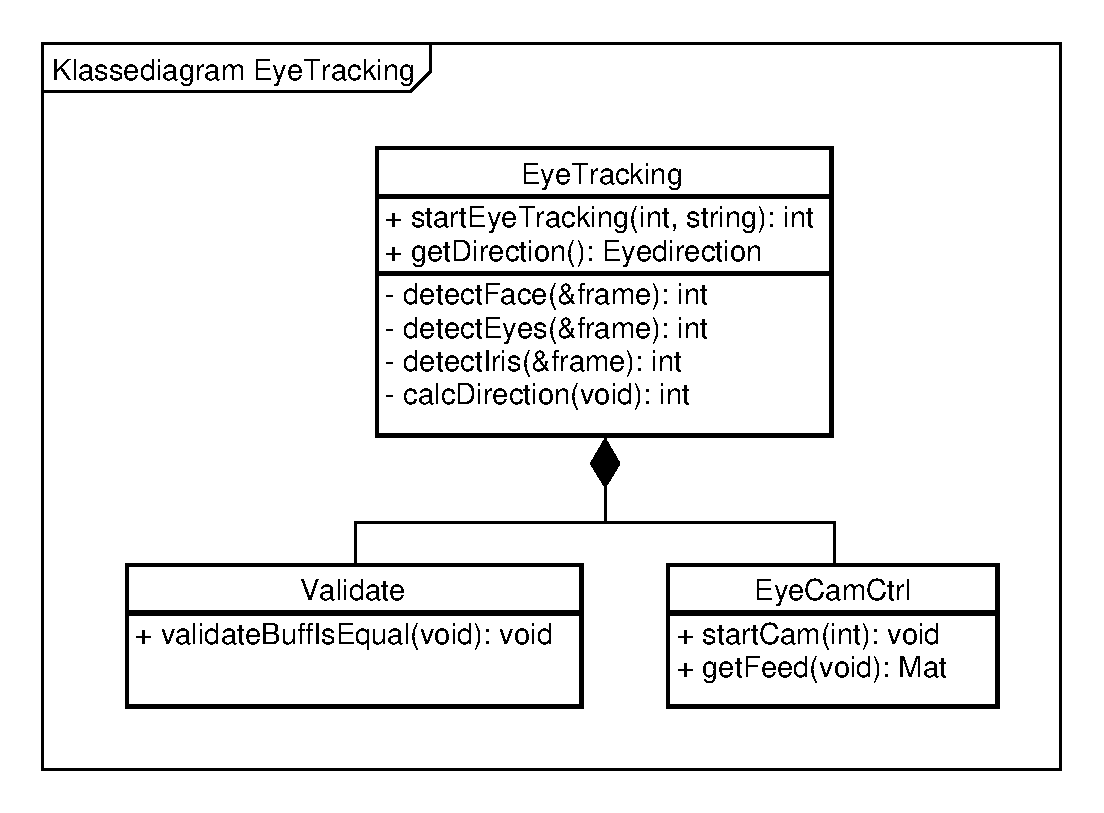
\includegraphics[width = 0.6\textwidth] {klasseEye.pdf}
	\captionof{figure}{Klassediagram over øjendetekteringsmodulet}
	\label{fig:eyeclass}
\end{figure}
 
EyeTracking indeholder initiering af modulet og hovedflowet, som er beskrevet i tidligere afsnit. 
Dette sker i funktionen startEyeTracking(). \\
Håndteringen af data er implementeret med STL containers.  
Dette er fordi detekteringerne ofte giver flere mulige kandidater til ansigter, øjne og iris. 
Der er derfor implementeret sorteringsalgoritmer baseret på STL funktionerne sort() og transform() for at sikre, at det er det ønskede detekterede objekt som vælges.
   
   
\subsection{Filtrering}
I Eyetrackingklassen bruges kun en brøkdel af den information, der findes i et frame. 
Derfor bruges der forskellige typer af filtreringsmetoder, så kun relevant data bibeholdes.

Den første behandling, der foretages, er en konvertering af farverne i billedet til gråtoner. 
Informationen i et farvebillede er delt ud på tre lag: rød, grøn og blå. 
For at kunne arbejde med framet, skal det samles til et enkelt lag. 
Dette gøres ved en gråtonekonvertering, hvor der foretages en vægtet sammensmeltning af de tre farvedimensioner.

Efterfølgende foretages yderligere filtrering af framet. 
Følgende filtreringsmetoder er testet:

\begin{itemize}
	\item Histogramnormalisering -	Breder histogrammet for billedets farveintensitetsdistribution ud over de mindre brugte intensiteter 
	\item Gaussisk udjævning - Folder billedet med en gaussisk funktion, der fungerer som et lavpasfilter, hvilket reducerer støjen.
	\item Kontrastforøgelse - Justerer kontrasten og lysstyrken i billedet.
\end{itemize}

Under test blev histogramnormalisering og gaussisk udjævning fravalgt, grundet en  høj bearbejdningstid, hvilket sænkede frameraten markant.\\
Under kontrastforøgelse foretages en direkte konvertering af billedet med convertTo-funktionen i OpenCV-biblioteket. 
Denne funktion ændrer billedet med en kontrastskaleringsfaktor, $ \alpha $, og en lysstyrkeskaleringsfaktor, $ \beta $.
Denne konvertering sker ved en lineær operation på de individuelle pixels, der er udformet som følger: 
\begin{equation}
	g(i,j) = \alpha \cdot f(i,j) + \beta
\end{equation}   
    
    
\subsection{Ansigts- og Øjendetektering}
For at behandle videoinputtet effektivt, bliver der foretaget flere operationer, som skærer unødvendig information fra framet. 
Først foretages en filtrering, som beskrivet i afsnittet "Filtrering", og derefter beskæres framet ind til områder med ansigts- og øjenobjekter.

Ved hjælp af ansigts- og øjengenkendelse, bliver området for brugerens position identificeret i det nuværende frame. Dette sker ved følgende fremgangsmåde: 

\begin{enumerate}
	\item Først detekteres ansigtet i framet 
	\item Framet beskæres til omkring ansigtet
	\item I det nu beskårne frame detekteres øjnene
	\item Framet beskæres yderligere ind til området omkring det ene øje
	\item Framet er klar til irisdetektering
\end{enumerate}

Kun ét øje er nødvendigt til at foretage en irisdetektering, da det antages, at brugerens øjne bevæger sig synkront. 
Derfor findes det største øje ved kalibreringen, som derefter bruges som det styrende øje. 
For at sørge for, at detekteringsfunktionen ikke skifter mellem brugerens øjne, bliver de fundne øjne i hvert frame sammenlignet med positionen fra den sidste øjendetektering. 

Selve ansigts- og øjengenkendelsen er implementeret ved brug af en classifier-caskade kaldt "Haar Feature-based Cascade Classifiers" \cite{MRL}. 
En classifier indeholder features, som er dominerende træk fra det objekt, der ønskes detekteret \cite{VIOLA}, som for eksempel et hovedomrids. 
Classifieren sammenligner disse features med framet og returnerer koordinaterne for matchene objekter. \\
Cascade Classifiers er opbygget af flere kaskadekoblede classifiers, for at optimere detekteringsprocessen. 
Bearbejdningstiden nedsættes ved at tage classifiers med få stærke features først, og derefter opjustere mængden af features i de efterfølgende classifiers.  
Det effektive består i, at billedbehandlingen bliver afsluttet, hvis der ikke er objektindikerende træk. 
Derved undgås det at spilde behandlingstid på uanvendelige frames.\\
En Classifier kan trænes ved at give den en stor mængde data i form af negative - og positive - træningssæt.
I Eyetrackingklassen bruges to Cascade classifiers, der er trænet på forhånd. Disse filer findes som standard i OpenCV-biblioteket.


\subsection{Iris detektering}
Denne funktion er implementeret med det formål at finde centrum af iris i et gråtonebillede, som har været igennem øjendetektering, og derfor er beskåret sådan, at kun det styrende øje er i framet. \\
Først behandles framet med et binært threshold filter.
Filterets funktion er at ændre alle pixels til sort, hvis dens værdi er under grænsen, ellers hvid. 
Grænseværdien bliver kalibreret i forhold til lysstyrken ved det første inputframe. 
Optimalt fjerner filtret alt andet end iris fra framet. 
Andre elementer af framet kan dog fremstå ligeså mørke, hvilket gør at de ikke fjernes. 

Det binære resultat sendes derefter videre til en formfindende algomitme.
Denne er i openCV implementeret i SimpleBlobDetector(). 
For at eliminere andre objekter end iris, er detekteringsalgoritmen opsat til at sammenligne objekter i framet efter størrelse og rundhed. \\
I projektet er "rundhedsparameteren" sat til en firkant. 
Hvis opløsningen på billedet var bedre, kunne den sættes til en cirkel. \\
Da refleksionen i et øje ofte vil fremstå som et hul er algoritmen sat til at acceptere, at de detekterede objekter ikke er massive.


\subsection{Enhedstest}
Øjendetekteringsmodulet er blevet enhedstestet, for at sikre, at performance lever op til kravet om at køre i realtid. 
Modulet er testet på tre områder:

\begin{itemize}
	\item Hastighed: Hvor mange frames pr. sekund (fps) kan modulet behandle
	\item Robusthed: Hvor mange resultater bliver beregnet i forhold til antal fps
	\item Pålidelighed: Hvor stor en del af resultaterne er korrekte
\end{itemize}

Der er ikke testet for robusthed under varierende lysforhold.
Dette er fordi denne udgave af softwaren ikke kan håndtere lysændringer godt nok til, at en sådan test vil give brugbar information. \\
Resultater for enhedstesten kan findes i bilag \ref{appendix:Bilag_enhedstest_eyetracking}

\subsubsection{Delkonklusion}
Øjendetektionsmodulets ansvarsområder er at detektere og kalkulere brugerens synsretning, for at omsætte dette til styringskoordinater til robotten. 
Funktionaliteten til at opnå dette er blevet implementeret.\\ 
Modulet har sorteringsmetoder til at håndtere flere ansigter, øjne og iriser i samme frame. 
Der er også integreret en simpel lysintensitetskalibrering.

Det kan konkluderes ud fra enhedstesten, at modulet har en virkningsgrad god nok til proof of concept, men ikke robusthed eller pålidelighed nok til praktisk brug.  

%\end{document}